% Created 2025-05-20 Sal 14:17
% Intended LaTeX compiler: pdflatex
\documentclass[./main.tex]{subfiles}
\usepackage[utf8]{inputenc}
\usepackage[T1]{fontenc}
\usepackage{graphicx}
\usepackage{grffile}
\usepackage{longtable}
\usepackage{wrapfig}
\usepackage{rotating}
\usepackage[normalem]{ulem}
\usepackage{amsmath}
\usepackage{textcomp}
\usepackage{amssymb}
\usepackage{capt-of}
\usepackage{hyperref}
\usepackage{pgfpages}
\usepackage{copyrightbox}
\setbeameroption{show notes}
\AtBeginSection[]{\begin{frame}[allowframebreaks]{Outline}\tableofcontents[currentsection]\end{frame}}
\usetheme{default}
\author{Baris Turan}
\date{\today}
\title{}
\title[Progress Report]{Progress Report}
\author[ITLR-DDSim]{Baris Turan}
\date{20 May 2025}
\hypersetup{
 pdfauthor={Baris Turan},
 pdftitle={},
 pdfkeywords={},
 pdfsubject={},
 pdfcreator={Emacs 27.1 (Org mode 9.3)}, 
 pdflang={English}}
\begin{document}

\maketitle

\section{Diffusion Models}
\label{sec:org530609e}
\begin{frame}[label={sec:org52a6a9a}]{Denoising Diffusion Probabistic Models}
\begin{itemize}
\item Forward Process:
\begin{itemize}
\item Starting from input \(\mathbf{x}_0\sim q(\mathbf{x}_0)\), successively add i.i.d. Gaussian noise according to:
\end{itemize}
\begin{equation*}
\mathbf{x}_t = \sqrt{1-\beta_t}\mathbf{x}_{t-1}+\sqrt{\beta_t}\mathbf{\epsilon}_t, \text{ }
\mathbf{\epsilon}_t\sim\mathcal{N}(0, \mathbf{I})
\end{equation*}
for \(t=1,2, \ldots,T\)
\begin{itemize}
\item Train neural network (usually UNet) to predict \(\mathbf{\epsilon}_t\) at a given timestep \(t\) given noisy image \(\mathbf{x}_t\).
\item Minimize
\end{itemize}
\begin{equation*}
      L=\left \lVert \epsilon - \epsilon_\theta(x_t, t)\right \rVert^2
\end{equation*}
\end{itemize}
\end{frame}
\begin{frame}[label={sec:orgbe203e9}]{Denoising Diffusion Probabilistic Models}
\begin{itemize}
\item Backward Process:
\begin{itemize}
\item Use the trained neural network to estimate \(q(\mathbf{x}_{t-1}|\mathbf{x}_t)\)
\item Starting from \(x_{T}\sim\mathcal{N}(0, \mathbf{I})\), successively denoise
\end{itemize}
the image as
\begin{equation*}
      x_{t-1}=\frac{1}{\sqrt{\alpha_t}}\left(\mathbf{x}_t-\frac{\beta_t}{\sqrt{1-\bar{\alpha}_t}}\right)+\sqrt{\beta_t}\mathbf{\epsilon}, 
      \text{ } \mathbf{\epsilon}\sim\mathcal{N}(0, \mathbf{I})
\end{equation*}
\end{itemize}
\end{frame}
\begin{frame}[label={sec:orgd0d5d51}]{Conditional vs. Unconditional Models}
\begin{itemize}
\item So far, we have been trying to estimate \(q(\mathbf{x}_0)\)
\item For real life applications, we want \(q(\mathbf{x}_0|y)\)
\item In image generation, y can be text, semantic map, a different image etc.
\item For flow problems:
\begin{itemize}
\item Boundary conditions
\item Sparse measurements
\item Information from governing equations
\item \ldots{}
\end{itemize}
\end{itemize}
\end{frame}
\begin{frame}[label={sec:orgee273ea}]{Example: DiffDA}
\begin{itemize}
\item Weather-scale data assimilation framework
\item Conditioned on sparse observations and predictions of a forecast model
\item Conditioning for sparse observations implemented by soft-masking
\end{itemize}
\begin{adjustbox}{width=\textwidth,totalheight=0.6\paperheight,keepaspectratio,center}
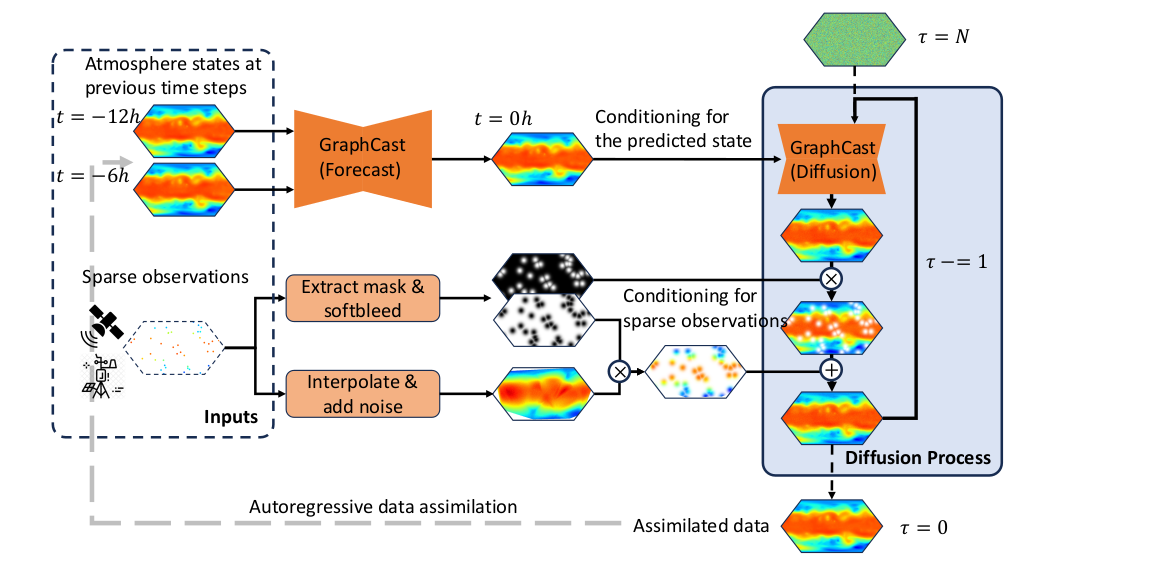
\includegraphics[width=\textwidth]{./figs/diffda.png}
\end{adjustbox}
\end{frame}
\begin{frame}[label={sec:org00bc5ad}]{Übung on Unconditional Diffusion Model}
\begin{itemize}
\item 2D homogeneous isotropic turbulence on 256x256 grid.
\item UNet architecture
\item Trained it on Google Colab for around 300 epochs
\end{itemize}
\begin{adjustbox}{width=\textwidth,totalheight=0.6\paperheight,keepaspectratio,center}
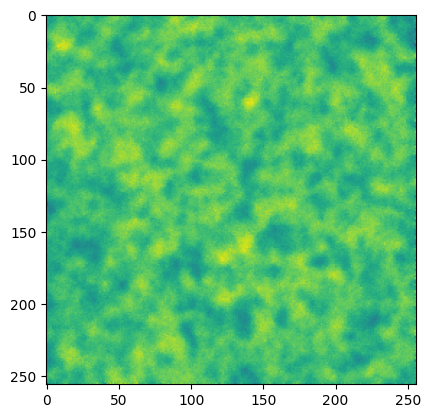
\includegraphics[width=\textwidth]{./figs/Kolmogorov3.png}
\end{adjustbox}
\end{frame}
\begin{frame}[label={sec:org5a9dfa2}]{Übung on Conditional Diffusion Model}
\begin{itemize}
\item Uses measurements in a random 50x50 region as condition.
\item Condition, timestep and noisy data are concatenated.
\item I used the pretrained model this time.
\end{itemize}
\begin{adjustbox}{width=\textwidth,totalheight=0.6\paperheight,keepaspectratio,center}
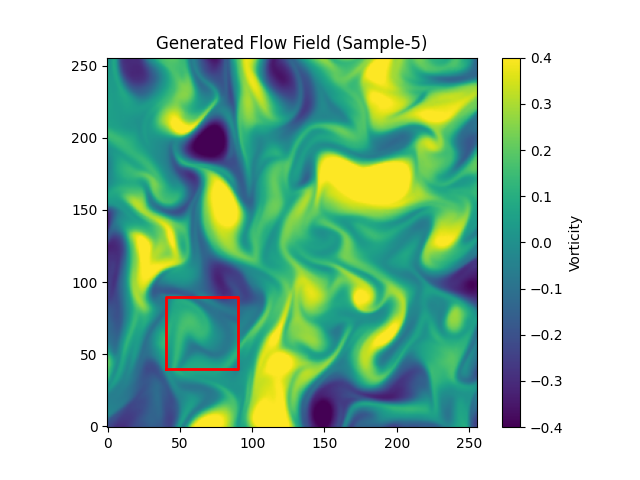
\includegraphics[width=\textwidth]{./figs/generated_image_5.png}
\end{adjustbox}
\end{frame}
\section{Stochastic Differential Equations}
\label{sec:org506e091}
\begin{frame}[label={sec:org5ef3c69}]{SDEs}
\begin{itemize}
\item Describe the time evolution of stochastic processes
\item General form is given by
\end{itemize}
\begin{equation*}
d\mathb{x}_t=\underbrace{\mathbf{\mu}(\mathbf{x}_t, t)dt}_{\text{Deterministic Part}}+\underbrace{\mathbf{\sigma}(\mathbf{x}_t, t)d\mathbf{w}_t}_{\text{Probabilistic Part}}.
\end{equation*}
\begin{itemize}
\item \(\mathbf{\mu}(\mathbf{x}_t, t)dt\): drift term
\item \(\mathbf{\sigma}(\mathbf{x}_t, t)\): diffusion term
\item Equivalent to PDE for the probability distribution (Fokker-Planck-Kolmogorov Equation):
\end{itemize}
\begin{equation*}
\frac{\partial}{\partial t}p(\mathbf{x}, t)=-\frac{\partial}{\partial x}\left[\mathbf{\mu}(\mathbf{x},t)p(\mathbf{x},t)\right]+\frac{\partial^2}{\partial\mathbf{x}^2}\left[\frac{1}{2}\mathbf{\sigma
}\mathbf{\sigma}^Tp(\mathbf{x},t)\right]
\end{equation*}
\end{frame}
\begin{frame}[label={sec:orgd14ed00}]{Diffusion Models as SDEs}
\begin{itemize}
\item SDE for forward diffusion:
\end{itemize}
\begin{equation*}
d\mathbf{x}=-\frac{1}{2}\beta_t\mathbf{x}dt+\sqrt{\beta_t}d\mathbf{w}
\end{equation*}
\begin{itemize}
\item SDE for backward diffusion:
\end{itemize}
\begin{equation*}
d\mathbf{x}=\left[-\frac{\beta_t}{2}-\beta_t\nabla_\mathbf{x} \log p(\mathbf{x})\right] + \sqrt{\beta_t}d\mathbf{w}
\end{equation*}
\begin{itemize}
\item \(s=\log p(\mathbf{x})\) is the score function.
\item \alert{Score based diffusion models} estimate the score function.
\item The SDE is then solved numerically using Euler-Maruyama integration
\end{itemize}
\end{frame}
\section{Variational Autoencoders (VAE)}
\label{sec:orga88d442}
\begin{frame}[label={sec:orgd79a8bb}]{Autoencoder}
\begin{itemize}
\item A network aiming to reconstruct the input
\begin{itemize}
\item Enconder: Compresses the input to the latent space
\item Decoder: Reconstructs input from the latent space representation.
\end{itemize}
\item Can be used for feature extraction
\item Decoder can potentially act as a generative model.
\end{itemize}
\begin{adjustbox}{width=\textwidth,totalheight=0.6\paperheight,keepaspectratio,center}
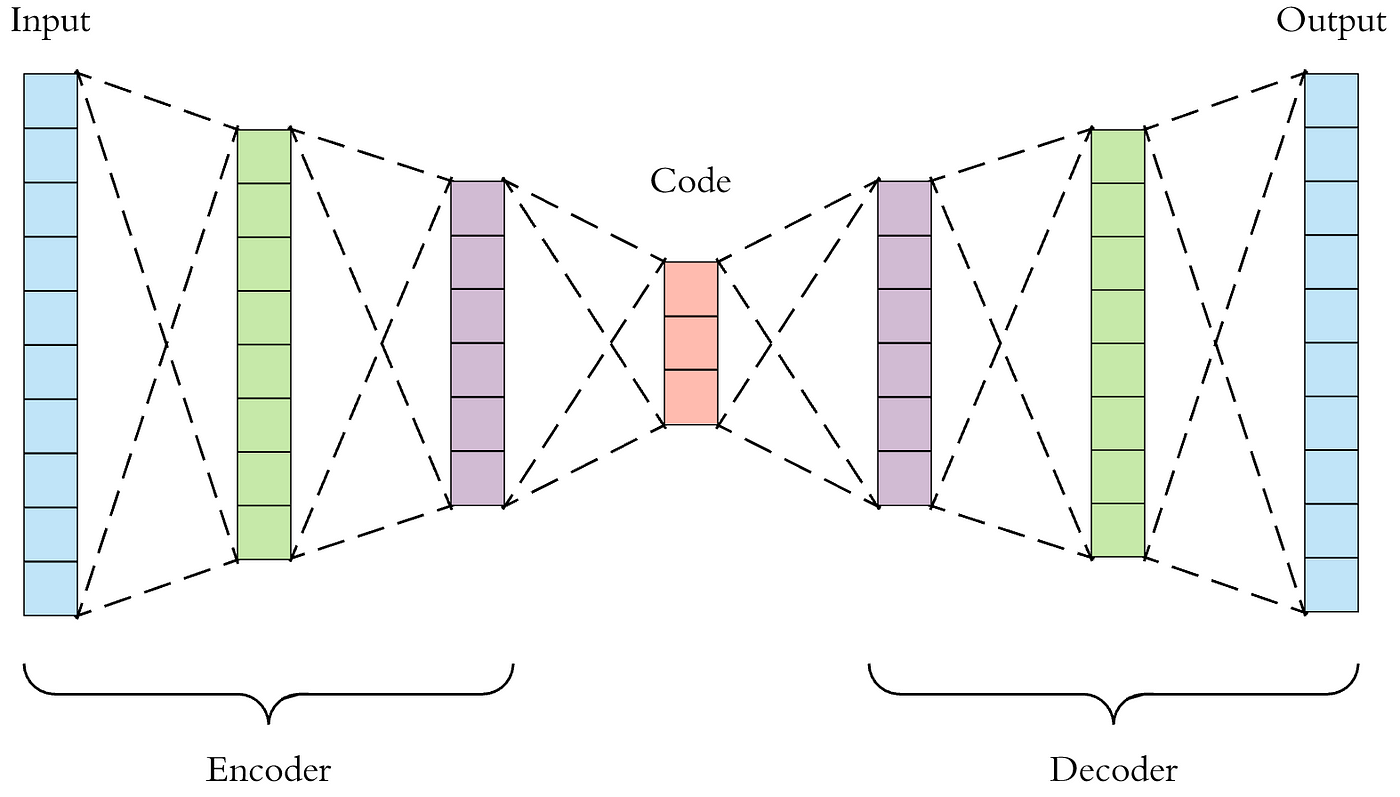
\includegraphics[width=\textwidth]{./figs/autoencoder.png}
\end{adjustbox}
\end{frame}
\begin{frame}[label={sec:orgf6035ca}]{VAE}
\begin{itemize}
\item Encoder maps input \(\mathbf{x}\) to a probability distribution \(p(\matbf{x}|\mathbf{z})\)
\item Decoder samples from this distribution and reconstructs the input
\item In addition to the usual L1 or L2 reconstruction loss, the loss function includes a KL divergenece term to make the distribution similar to \(\mathcal{N}(0, \mathbf{I})\)
\item Latent space is more centered and regularized, so better for generative tasks than vanilla AE.
\end{itemize}
\begin{columns}
\begin{column}{0.5\columnwidth}
\begin{adjustbox}{width=\textwidth,totalheight=0.6\paperheight,keepaspectratio,center}
\includegraphics[width=\textwidth]{./figs/AE_Latent_Space.png}
\end{adjustbox}
\end{column}

\begin{column}{0.5\columnwidth}
\begin{adjustbox}{width=\textwidth,totalheight=0.6\paperheight,keepaspectratio,center}
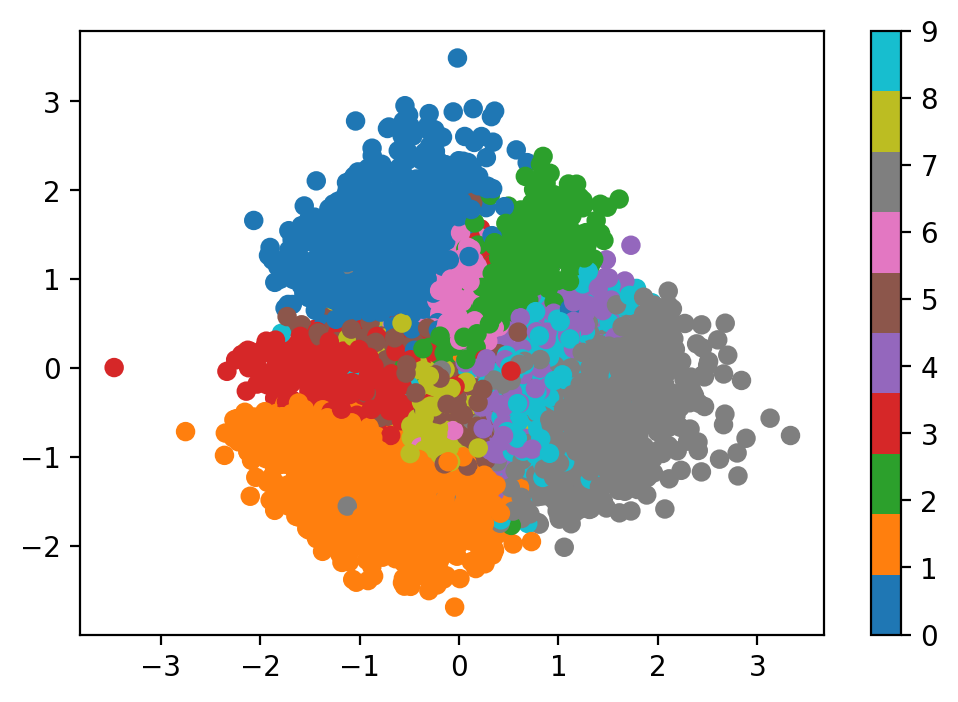
\includegraphics[width=\textwidth]{./figs/VAE_Latent_Space.png}
\end{adjustbox}
\end{column}
\end{columns}
\end{frame}

\section{Stable Diffusion}
\label{sec:org865b3b1}
\begin{frame}[label={sec:org795fef4}]{Stable Diffusion}
\begin{itemize}
\item Uses a VAE to compress the data into latent space
\item Diffusion is carried out in latent space to reduce computational costs
\item Uses attention for conditionin.
\end{itemize}
\begin{adjustbox}{width=\textwidth,totalheight=0.6\paperheight,keepaspectratio,center}
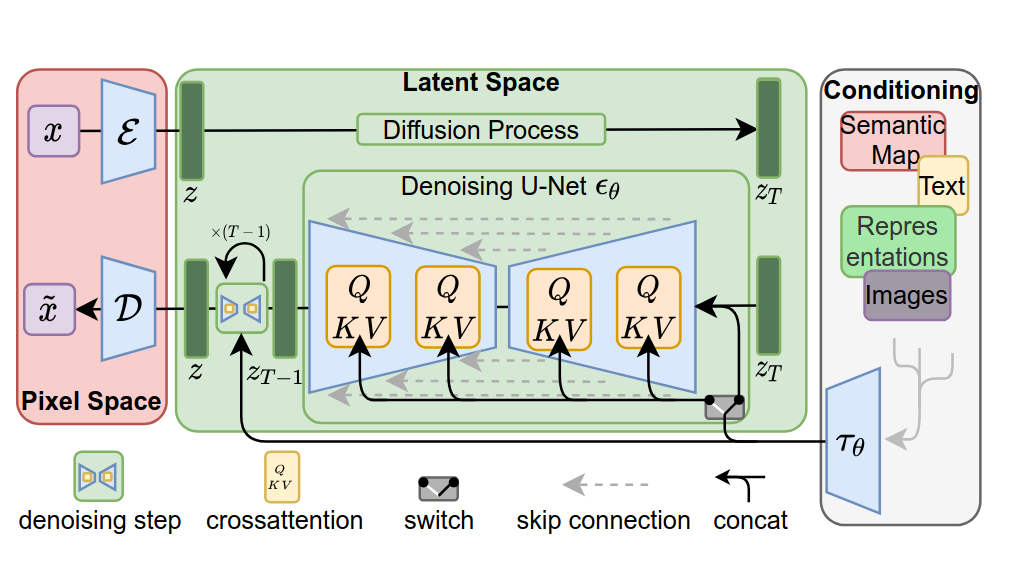
\includegraphics[width=\textwidth]{./figs/stable_diffusion.png}
\end{adjustbox}
\end{frame}
\section{Summary}
\label{sec:org89ae61b}
\begin{frame}[label={sec:org7b8dd0c}]{Summary}
\begin{itemize}
\item I have read about diffusion models, SDEs, VAEs
\item I have done the Übungs on diffusion models
\end{itemize}
\end{frame}

\section{Plan for This Week}
\label{sec:org685f34f}
\begin{frame}[label={sec:org7a954be}]{Plan for This Week}
\begin{itemize}
\item Read Hao's windfarm proposal
\item Work on conditioning based on energy spectrum, two-point correlation
\item Help Fabian with the urban heat island problem
\end{itemize}
\end{frame}
\end{document}
